\q{15}{Search}
\begin{center}
\begin{tabular}{cc}
\parbox[c]{10cm}{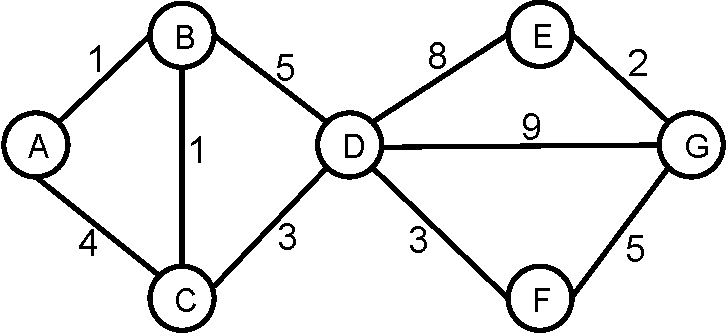
\includegraphics[width =0.6\linewidth]{figs/search_graph.pdf}}
&
\begin{tabular}[h]{|c|c|c|}
\hline
Node &$h_1$ 	&	$h_2$ \\
\hline
A 	& 	9.5 	&	10 	\\
B 	&	9	&	12	\\
C 	&	8	&	10	\\
D 	&	7	&	8	\\
E 	&	1.5	&	1	\\
F 	&	4	&	4.5	\\
G 	&	0	&	0	\\
\hline 
\end{tabular}
\end{tabular}
\end{center}

Consider the state space graph shown above.  A is the start state and
G is the goal state. The costs for each edge are shown on the graph.  Each edge can
be traversed in both directions.   Note that the heuristic $h_1$ is consistent
but the heuristic $h_2$ is not consistent.  

%%PA: I added the info about consistency of the heuristics, as this
%%way (a) students who understand the consequences can more quickly
%%answer the question that involves h1; (b) students who would just simply mark the
%%shortest whenever asked about A* might now have to think more
%%properly through what happens for h2

\begin{question}[6] \textbf{Possible paths returned} {
For each of the following graph search strategies (\emph{do not answer for tree search}), mark which, if any, of the
listed paths it could return.   Note that for some search strategies
the specific path returned might depend on tie-breaking behavior.   In any such cases, make sure to mark
}
\emph{all} paths that could be returned under some tie-breaking scheme.
\vspace{.1in}
\begin{table}[!h]
\centering
\begin{tabular}{|l|l|l|l|}
\hline
Search Algorithm &  \textbf{A-B-D-G} & \textbf{A-C-D-G} &
\textbf{A-B-C-D-F-G} \\
\hline
Depth first search & (i) \AnswerTwoAi & (ii) \AnswerTwoAii & (iii) \AnswerTwoAiii \\
\hline
Breadth first search & (iv) \AnswerTwoAiv & (v) \AnswerTwoAv & (vi) \AnswerTwoAvi \\
\hline
Uniform cost search & (vii) \AnswerTwoAvii & (viii) \AnswerTwoAviii & (ix) \AnswerTwoAix \\
\hline
A* search with heuristic $h_1$ & (x) \AnswerTwoAx & (xi) \AnswerTwoAxi & (xii) \AnswerTwoAxii \\
\hline
A* search with heuristic $h_2$ & (xiii) \AnswerTwoAxiii & (xiv) \AnswerTwoAxiv & (xv) \AnswerTwoAxv \\
\hline
\end{tabular}
\end{table}


\end{question}

\begin{question}[] \textbf{Heuristic function properties}\\
Suppose you are completing the new heuristic function $h_3$ shown below.
All the values are fixed except $h_3(B)$.  


\begin{center}

\begin{tabular}{|c|c|c|c|c|c|c|c|}
\hline
Node & A & B & C & D & E & F & G \\
\hline
$h_3$& 10 & ?  & 9 & 7 & 1.5 & 4.5& 0 \\
\hline
\end{tabular}
\end{center}

For each of the following conditions, write the set
of values that are possible for $h_3(B)$.
For example, to denote all non-negative numbers, write [0, $\infty$], to denote the empty set, write $\varnothing$, and so on.

\vspace{0.5 cm}
\begin{subquestion}[2]
\textbf{What values of $h_3(B)$ make $h_3$ admissible?} \\
\fbox{\begin{minipage}[t][2cm][t]{13cm} \AnswerTwoBi \end{minipage}} \\

\end{subquestion}

\begin{subquestion}[3]
\textbf{What values of $h_3(B)$ make $h_3$ consistent?} \\
\fbox{\begin{minipage}[t][2cm][t]{13cm} \AnswerTwoBii \end{minipage}} \\


\end{subquestion}

\begin{subquestion}[4]
\textbf{What values of $h_3(B)$ will cause A* graph search to expand node A, then node C, then node B, then node D in order?} \\
\fbox{\begin{minipage}[t][2cm][t]{13cm} \AnswerTwoBiii \end{minipage}} \\

\end{subquestion}
%%PA: I changed the answer to be 12<h_3(B)<14 (from 12<h_3(B)<13)

\end{question}








